% I seguenti commenti speciali impostano:
% 1. 
% 2. PDFLaTeX come motore di composizione;
% 3. tesi.tex come documento principale;
% 4. il controllo ortografico italiano per l'editor.

% !TEX encoding = UTF-8
% !TEX TS-program = pdflatex
% !TEX root = tesi.tex
% !TEX spellcheck = it-IT

% PDF/A filecontents
\RequirePackage{filecontents}
\begin{filecontents*}{\jobname.xmpdata}
  \Title{Document’s title}
  \Author{Author’s name}
  \Language{it-IT}
  \Subject{The abstract, or short description.}
  \Keywords{keyword1\sep keyword2\sep keyword3}
\end{filecontents*}

\documentclass[10pt,                    % corpo del font principale
               a4paper,                 % carta A4
               twoside,                 % impagina per fronte-retro
               openright,               % inizio capitoli a destra
               english,                 
               italian,                 
               ]{book}    

%**************************************************************
% Importazione package
%************************************************************** 

\PassOptionsToPackage{dvipsnames}{xcolor} % colori PDF/A

\usepackage{colorprofiles}

\usepackage[a-2b,mathxmp]{pdfx}[2018/12/22]
                                        % configurazione PDF/A
                                        % validare in https://www.pdf-online.com/osa/validate.aspx

%\usepackage{amsmath,amssymb,amsthm}    % matematica

\usepackage[T1]{fontenc}                % codifica dei font:
                                        % NOTA BENE! richiede una distribuzione *completa* di LaTeX

\usepackage[utf8]{inputenc}             % codifica di input; anche [latin1] va bene
                                        % NOTA BENE! va accordata con le preferenze dell'editor

\usepackage[english, italian]{babel}    % per scrivere in italiano e in inglese;
                                        % l'ultima lingua (l'italiano) risulta predefinita
       
\usepackage[mediumspace,mediumqspace,Grey,squaren]{SIunits}  % unità di misura                                   

\usepackage{bookmark}                   % segnalibri

\usepackage{algorithm}
\usepackage[noend]{algpseudocode}

\usepackage{caption}                    % didascalie

\usepackage{chngpage,calc}              % centra il frontespizio

\usepackage{csquotes}                   % gestisce automaticamente i caratteri (")

\usepackage{emptypage}                  % pagine vuote senza testatina e piede di pagina

\usepackage{epigraph}			% per epigrafi

\usepackage{eurosym}                    % simbolo dell'euro

%\usepackage{indentfirst}               % rientra il primo paragrafo di ogni sezione

\usepackage{graphicx}                   % immagini

\usepackage{hyperref}                   % collegamenti ipertestuali

\usepackage[binding=5mm]{layaureo}      % margini ottimizzati per l'A4; rilegatura di 5 mm

\usepackage{listings}                   % codici

\usepackage{microtype}                  % microtipografia

\usepackage{mparhack,fixltx2e,relsize}  % finezze tipografiche

\usepackage{nameref}                    % visualizza nome dei riferimenti                                      
\usepackage[font=small]{quoting}        % citazioni

\usepackage{subfig}                     % sottofigure, sottotabelle

\usepackage[italian]{varioref}          % riferimenti completi della pagina

\usepackage{booktabs}                   % tabelle                                       
\usepackage{tabularx}                   % tabelle di larghezza prefissata                                    
\usepackage{longtable}                  % tabelle su più pagine                                        
\usepackage{ltxtable}                   % tabelle su più pagine e adattabili in larghezza

\usepackage{textcomp}                   % trademark
\usepackage{listings}                   % for matlab code

\usepackage[toc, acronym]{glossaries}   % glossario
                                        % per includerlo nel documento bisogna:
                                        % 1. compilare una prima volta tesi.tex;
                                        % 2. eseguire: makeindex -s tesi.ist -t tesi.glg -o tesi.gls tesi.glo
                                        % 3. eseguire: makeindex -s tesi.ist -t tesi.alg -o tesi.acr tesi.acn
                                        % 4. compilare due volte tesi.tex.

\usepackage[backend=biber,style=verbose-ibid,hyperref,backref]{biblatex}
                                        % eccellente pacchetto per la bibliografia; 
                                        % produce uno stile di citazione autore-anno; 
                                        % lo stile "numeric-comp" produce riferimenti numerici
                                        % per includerlo nel documento bisogna:
                                        % 1. compilare una prima volta tesi.tex;
                                        % 2. eseguire: biber tesi
                                        % 3. compilare ancora tesi.tex.
                                        
%**************************************************************
% file contenente le impostazioni della tesi
%**************************************************************

%**************************************************************
% Frontespizio
%**************************************************************

% Autore
\newcommand{\myName}{Riccardo Montagnin}                                    
\newcommand{\myTitle}{Titolo della tesi}

% Tipo di tesi                   
\newcommand{\myDegree}{Tesi di laurea}

% Università             
\newcommand{\myUni}{Università degli Studi di Padova}

% Facoltà       
\newcommand{\myFaculty}{Corso di Laurea in Informatica}

% Dipartimento
\newcommand{\myDepartment}{Dipartimento di Matematica "Tullio Levi-Civita"}

% Titolo del relatore
\newcommand{\profTitle}{Prof.}

% Relatore
\newcommand{\myProf}{Tullio Vardanega}

% Luogo
\newcommand{\myLocation}{Padova}

% Anno accademico
\newcommand{\myAA}{2016-2017}

% Data discussione
\newcommand{\myTime}{Luglio 2017}


%**************************************************************
% Impostazioni di impaginazione
% see: http://wwwcdf.pd.infn.it/AppuntiLinux/a2547.htm
%**************************************************************

\setlength{\parindent}{14pt}   % larghezza rientro della prima riga
\setlength{\parskip}{0pt}   % distanza tra i paragrafi


%**************************************************************
% Impostazioni di biblatex
%**************************************************************
\bibliography{bibliografia} % database di biblatex 

\defbibheading{bibliography} {
    \cleardoublepage
    \phantomsection 
    \addcontentsline{toc}{chapter}{\bibname}
    \chapter*{\bibname\markboth{\bibname}{\bibname}}
}

\setlength\bibitemsep{1.5\itemsep} % spazio tra entry

\DeclareBibliographyCategory{opere}
\DeclareBibliographyCategory{web}

\addtocategory{opere}{womak:lean-thinking}
\addtocategory{web}{site:agile-manifesto}

\defbibheading{opere}{\section*{Riferimenti bibliografici}}
\defbibheading{web}{\section*{Siti Web consultati}}


%**************************************************************
% Impostazioni di caption
%**************************************************************
\captionsetup{
    tableposition=top,
    figureposition=bottom,
    font=small,
    format=hang,
    labelfont=bf
}

%**************************************************************
% Impostazioni di glossaries
%**************************************************************

%**************************************************************
% Acronimi
%**************************************************************
\renewcommand{\acronymname}{Acronimi e abbreviazioni}

\newacronym[description={\glslink{apig}{Application Program Interface}}]
    {api}{API}{Application Program Interface}

\newacronym[description={\glslink{umlg}{Unified Modeling Language}}]
    {uml}{UML}{Unified Modeling Language}

%**************************************************************
% Glossario
%**************************************************************
%\renewcommand{\glossaryname}{Glossario}

\newglossaryentry{apig}
{
    name=\glslink{api}{API},
    text=Application Program Interface,
    sort=api,
    description={in informatica con il termine \emph{Application Programming Interface API} (ing. interfaccia di programmazione di un'applicazione) si indica ogni insieme di procedure disponibili al programmatore, di solito raggruppate a formare un set di strumenti specifici per l'espletamento di un determinato compito all'interno di un certo programma. La finalità è ottenere un'astrazione, di solito tra l'hardware e il programmatore o tra software a basso e quello ad alto livello semplificando così il lavoro di programmazione}
}

\newglossaryentry{umlg}
{
    name=\glslink{uml}{UML},
    text=UML,
    sort=uml,
    description={in ingegneria del software \emph{UML, Unified Modeling Language} (ing. linguaggio di modellazione unificato) è un linguaggio di modellazione e specifica basato sul paradigma object-oriented. L'\emph{UML} svolge un'importantissima funzione di ``lingua franca'' nella comunità della progettazione e programmazione a oggetti. Gran parte della letteratura di settore usa tale linguaggio per descrivere soluzioni analitiche e progettuali in modo sintetico e comprensibile a un vasto pubblico}
}
 % database di termini
\makeglossaries


%**************************************************************
% Impostazioni di graphicx
%**************************************************************
\graphicspath{{immagini/}} % cartella dove sono riposte le immagini


%**************************************************************
% Impostazioni di hyperref
%**************************************************************
\hypersetup{
    %hyperfootnotes=false,
    %pdfpagelabels,
    %draft,	% = elimina tutti i link (utile per stampe in bianco e nero)
    colorlinks=true,
    linktocpage=true,
    pdfstartpage=1,
    pdfstartview=,
    % decommenta la riga seguente per avere link in nero (per esempio per la stampa in bianco e nero)
    %colorlinks=false, linktocpage=false, pdfborder={0 0 0}, pdfstartpage=1, pdfstartview=FitV,
    breaklinks=true,
    pdfpagemode=UseNone,
    pageanchor=true,
    pdfpagemode=UseOutlines,
    plainpages=false,
    bookmarksnumbered,
    bookmarksopen=true,
    bookmarksopenlevel=1,
    hypertexnames=true,
    pdfhighlight=/O,
    %nesting=true,
    %frenchlinks,
    urlcolor=webbrown,
    linkcolor=RoyalBlue,
    citecolor=webgreen,
    %pagecolor=RoyalBlue,
    %urlcolor=Black, linkcolor=Black, citecolor=Black, %pagecolor=Black,
    pdftitle={\myTitle},
    pdfauthor={\textcopyright\ \myName, \myUni, \myFaculty},
    pdfsubject={},
    pdfkeywords={},
    pdfcreator={pdfLaTeX},
    pdfproducer={LaTeX}
}

%**************************************************************
% Impostazioni di itemize
%**************************************************************
\renewcommand{\labelitemi}{$\ast$}

%\renewcommand{\labelitemi}{$\bullet$}
%\renewcommand{\labelitemii}{$\cdot$}
%\renewcommand{\labelitemiii}{$\diamond$}
%\renewcommand{\labelitemiv}{$\ast$}


%**************************************************************
% Impostazioni di listings
%**************************************************************
\lstset{
    language=[LaTeX]Tex,%C++,
    keywordstyle=\color{RoyalBlue}, %\bfseries,
    basicstyle=\small\ttfamily,
    %identifierstyle=\color{NavyBlue},
    commentstyle=\color{Green}\ttfamily,
    stringstyle=\rmfamily,
    numbers=none, %left,%
    numberstyle=\scriptsize, %\tiny
    stepnumber=5,
    numbersep=8pt,
    showstringspaces=false,
    breaklines=true,
    frameround=ftff,
    frame=single
} 


%**************************************************************
% Impostazioni di xcolor
%**************************************************************
\definecolor{webgreen}{rgb}{0,.5,0}
\definecolor{webbrown}{rgb}{.6,0,0}


%**************************************************************
% Altro
%**************************************************************

\newcommand{\omissis}{[\dots\negthinspace]} % produce [...]

% eccezioni all'algoritmo di sillabazione
\hyphenation
{
    ma-cro-istru-zio-ne
    gi-ral-din
}

\newcommand{\sectionname}{sezione}
\addto\captionsitalian{\renewcommand{\figurename}{Figura}
                       \renewcommand{\tablename}{Tabella}}

\newcommand{\glsfirstoccur}{\ap{{[g]}}}

\newcommand{\intro}[1]{\emph{\textsf{#1}}}

%**************************************************************
% Environment per ``rischi''
%**************************************************************
\newcounter{riskcounter}                % define a counter
\setcounter{riskcounter}{0}             % set the counter to some initial value

%%%% Parameters
% #1: Title
\newenvironment{risk}[1]{
    \refstepcounter{riskcounter}        % increment counter
    \par \noindent                      % start new paragraph
    \textbf{\arabic{riskcounter}. #1}   % display the title before the 
                                        % content of the environment is displayed 
}{
    \par\medskip
}

\newcommand{\riskname}{Rischio}

\newcommand{\riskdescription}[1]{\textbf{\\Descrizione:} #1.}

\newcommand{\risksolution}[1]{\textbf{\\Soluzione:} #1.}

%**************************************************************
% Environment per ``use case''
%**************************************************************
\newcounter{usecasecounter}             % define a counter
\setcounter{usecasecounter}{0}          % set the counter to some initial value

%%%% Parameters
% #1: ID
% #2: Nome
\newenvironment{usecase}[2]{
    \renewcommand{\theusecasecounter}{\usecasename #1}  % this is where the display of 
                                                        % the counter is overwritten/modified
    \refstepcounter{usecasecounter}             % increment counter
    \vspace{10pt}
    \par \noindent                              % start new paragraph
    {\large \textbf{\usecasename #1: #2}}       % display the title before the 
                                                % content of the environment is displayed 
    \medskip
}{
    \medskip
}

\newcommand{\usecasename}{UC}

\newcommand{\usecaseactors}[1]{\textbf{\\Attori Principali:} #1. \vspace{4pt}}
\newcommand{\usecasepre}[1]{\textbf{\\Precondizioni:} #1. \vspace{4pt}}
\newcommand{\usecasedesc}[1]{\textbf{\\Descrizione:} #1. \vspace{4pt}}
\newcommand{\usecasepost}[1]{\textbf{\\Postcondizioni:} #1. \vspace{4pt}}
\newcommand{\usecasealt}[1]{\textbf{\\Scenario Alternativo:} #1. \vspace{4pt}}

%**************************************************************
% Environment per ``namespace description''
%**************************************************************

\newenvironment{namespacedesc}{
    \vspace{10pt}
    \par \noindent                              % start new paragraph
    \begin{description} 
}{
    \end{description}
    \medskip
}

\newcommand{\classdesc}[2]{\item[\textbf{#1:}] #2}
                     % file con le impostazioni personali

\begin{document}
%**************************************************************
% Materiale iniziale
%**************************************************************
\frontmatter
% !TEX encoding = UTF-8
% !TEX TS-program = pdflatex
% !TEX root = ../tesi.tex

%**************************************************************
% Frontespizio 
%**************************************************************
\begin{titlepage}

\begin{center}

\begin{LARGE}
\textbf{\myUni}\\
\end{LARGE}

\vspace{10pt}

\begin{Large}
\textsc{\myDepartment}\\
\end{Large}

\vspace{10pt}

\begin{large}
\textsc{\myFaculty}\\
\end{large}

\vspace{30pt}
\begin{figure}[htbp]
\begin{center}

\includegraphics[height=6cm]{logo-unipd}
\end{center}
\end{figure}
\vspace{30pt} 

\begin{LARGE}
\begin{center}
\textbf{\myTitle}\\
\end{center}
\end{LARGE}

\vspace{10pt} 

\begin{large}
\textsl{\myDegree}\\
\end{large}

\vspace{40pt} 

\begin{large}
\begin{flushleft}
\textit{Relatore}\\ 
\vspace{5pt} 
\profTitle \myProf
\end{flushleft}

\vspace{0pt} 

\begin{flushright}
\textit{Laureando}\\ 
\vspace{5pt} 
\myName
\end{flushright}
\end{large}

\vspace{40pt}

\line(1, 0){338} \\
\begin{normalsize}
\textsc{Anno Accademico \myAA}
\end{normalsize}

\end{center}
\end{titlepage} 
% !TEX encoding = UTF-8
% !TEX TS-program = pdflatex
% !TEX root = ../tesi.tex

%**************************************************************
% Colophon
%**************************************************************
\clearpage
\phantomsection
\thispagestyle{empty}

\hfill

\vfill

\noindent\myName: \textit{\myTitle,}
\myDegree,
\textcopyright\ \myTime.
% !TEX encoding = UTF-8
% !TEX TS-program = pdflatex
% !TEX root = ../tesi.tex

%**************************************************************
% Dedica
%**************************************************************
\cleardoublepage
\phantomsection
\thispagestyle{empty}
\pdfbookmark{Dedica}{Dedica}

\vspace*{3cm}

\begin{center}
If people do not believe that mathematics is simple, it is only because they do not realize how complicated life is.
\\ \medskip
--- John von Neumann
\end{center}

\medskip

% !TEX encoding = UTF-8
% !TEX TS-program = pdflatex
% !TEX root = ../tesi.tex

%**************************************************************
% Sommario
%**************************************************************
\cleardoublepage
\phantomsection
\pdfbookmark{Sommario}{Sommario}
\begingroup
\let\clearpage\relax
\let\cleardoublepage\relax
\let\cleardoublepage\relax

\chapter*{Sommario}

Il presente documento descrive il lavoro svolto durante il periodo di stage, della durata di circa 320 ore, dal laureando Michele Veronesi presso l'azienda IM4DIGITAL s.r.l.\\
Il focus del progetto di stage era lo studio di fattibilità di un sistema di navigazione per droni ricognitivi che decidesse la rotta in base allo spettro luminoso degli oggetti sorvolati.\\
In particolare, è stato necessario inizialmente identificare il dataset su cui fare lo studio, successivamente si è rivelata fondamentale la pulizia di questo.
Poi è stato richiesto di prendere in considerazione diversi modelli di machine learning e analizzare le prestazioni nel classificare gli oggetti tramite le loro firme spettrali,
in modo da selezionare il più adatto.
Infine il modello allenato è stato caricato ed esposto su infrastruttura cloud, con cui si è interfacciata la business logic che effettua il calcolo del percorso (anch'essa realizzata nel corso del tirocinio).\\
La suddivisione in capitoli è la seguente:
\begin{description}
    \item[{\hyperref[cap:introduzione]{Il primo capitolo}}] presenta la realtà aziendale e gli obiettivi dello stage.
    
    \item[{\hyperref[cap:machine-learning]{Il secondo capitolo}}] descrive nel dettaglio la parte di machine learning e analisi dei dati.
    
    \item[{\hyperref[cap:business-logic]{Il terzo capitolo}}] racconta la realizzazione della business logic per il calcolo della traiettoria del drone.
    
    \item[{\hyperref[cap:conclusione]{Il quarto capitolo}}], infine, porta una valutazione retrospettiva delle attività svolte e alcune considerazioni finali.
\end{description}
%\vfill
%
%\selectlanguage{english}
%\pdfbookmark{Abstract}{Abstract}
%\chapter*{Abstract}
%
%\selectlanguage{italian}

\endgroup			

\vfill


% !TEX encoding = UTF-8
% !TEX TS-program = pdflatex
% !TEX root = ../tesi.tex

%**************************************************************
% Ringraziamenti
%**************************************************************
\cleardoublepage
\phantomsection
\pdfbookmark{Ringraziamenti}{ringraziamenti}

\bigskip

\begingroup
\let\clearpage\relax
\let\cleardoublepage\relax
\let\cleardoublepage\relax

\chapter*{Ringraziamenti}

\noindent \textit{Innanzitutto, vorrei esprimere la mia gratitudine al Prof. Francesco Ranzato, relatore della mia tesi, per l'aiuto e il sostegno fornitomi durante la stesura del lavoro e della tesi.}\\

\noindent \textit{Desidero ringraziare con affetto i miei genitori e tutti i parenti per il sostegno, il grande aiuto e per essermi stati vicini in ogni momento durante gli anni di studio.}\\

\noindent \textit{Ho desiderio di ringraziare poi i miei studenti dell'istituto Nightingale, che hanno alleviato un periodo difficile con la loro solarità.}\\
\bigskip

\noindent\textit{\myLocation, \myTime}
\hfill \myName

\endgroup


% !TEX encoding = UTF-8
% !TEX TS-program = pdflatex
% !TEX root = ../tesi.tex

%**************************************************************
% Indici
%**************************************************************
\cleardoublepage
\pdfbookmark{\contentsname}{tableofcontents}
\setcounter{tocdepth}{2}
\tableofcontents
%\markboth{\contentsname}{\contentsname} 
\clearpage

\begingroup 
    \let\clearpage\relax
    \let\cleardoublepage\relax
    \let\cleardoublepage\relax
    %*******************************************************
    % Elenco delle figure
    %*******************************************************    
    \phantomsection
    \pdfbookmark{\listfigurename}{lof}
    \listoffigures

    \vspace*{8ex}

    %*******************************************************
    % Elenco delle tabelle
    %*******************************************************
    %\phantomsection
    %\pdfbookmark{\listtablename}{lot}
    %\listoftables
        
    \vspace*{8ex}
\endgroup

\cleardoublepage

\cleardoublepage

%**************************************************************
% Materiale principale
%**************************************************************
\mainmatter
% !TEX encoding = UTF-8
% !TEX TS-program = pdflatex
% !TEX root = ../tesi.tex

%**************************************************************
\chapter{Introduzione}
\label{cap:introduzione}
%**************************************************************

Introduzione al contesto applicativo.\\

\noindent Esempio di utilizzo di un termine nel glossario \\
\gls{api}. \\

\noindent Esempio di citazione in linea \\
\cite{site:agile-manifesto}. \\

\noindent Esempio di citazione nel pie' di pagina \\
citazione\footcite{womak:lean-thinking} \\

%**************************************************************
\section{L'azienda}

Descrizione dell'azienda.

%**************************************************************
\section{L'idea}

Introduzione all'idea dello stage.

%**************************************************************
\section{Organizzazione del testo}

\begin{description}
    \item[{\hyperref[cap:processi-metodologie]{Il secondo capitolo}}] descrive ...
    
    \item[{\hyperref[cap:descrizione-stage]{Il terzo capitolo}}] approfondisce ...
    
    \item[{\hyperref[cap:analisi-requisiti]{Il quarto capitolo}}] approfondisce ...
    
    \item[{\hyperref[cap:progettazione-codifica]{Il quinto capitolo}}] approfondisce ...
    
    \item[{\hyperref[cap:verifica-validazione]{Il sesto capitolo}}] approfondisce ...
    
    \item[{\hyperref[cap:conclusioni]{Nel settimo capitolo}}] descrive ...
\end{description}

Riguardo la stesura del testo, relativamente al documento sono state adottate le seguenti convenzioni tipografiche:
\begin{itemize}
	\item gli acronimi, le abbreviazioni e i termini ambigui o di uso non comune menzionati vengono definiti nel glossario, situato alla fine del presente documento;
	\item per la prima occorrenza dei termini riportati nel glossario viene utilizzata la seguente nomenclatura: \emph{parola}\glsfirstoccur;
	\item i termini in lingua straniera o facenti parti del gergo tecnico sono evidenziati con il carattere \emph{corsivo}.
\end{itemize}             % introduzione
% !TEX encoding = UTF-8
% !TEX TS-program = pdflatex
% !TEX root = ../tesi.tex

%**************************************************************
\chapter{Dataset e modello di machine learning}
\label{cap:machine-learning}
%**************************************************************

\intro{In questo capitolo si andrà a descrivere il dataset utilizzato, la sua elaborazione e lo sviluppo del modello di machine learning.}\\

%**************************************************************
\section{Descrizione del dataset}
\subsection{Descrizione del tipo di dati ricercati}
Dopo l'incontro con un esperto in geologia, a cui l'azienda si è rivolta per una consulenza, si è deciso di descrivere gli esempi che andranno in input al modello di machine learning attraverso la loro firma spettrale.
La firma spettrale è una caratteristica che ogni materiale ha, ed è specifica per ogni combinazione di riflessi e assorbimenti delle radiazioni elettromagnetiche (EM) a diverse lunghezze d'onda. Conoscendo la firma spettrale di un oggetto, è possibile identificarlo univocamente.
Un esempio di firma è quello riportato nella figura \ref{esempio_firma}, presa dal dataset di seguito presentato.
\begin{figure}
    \centering
    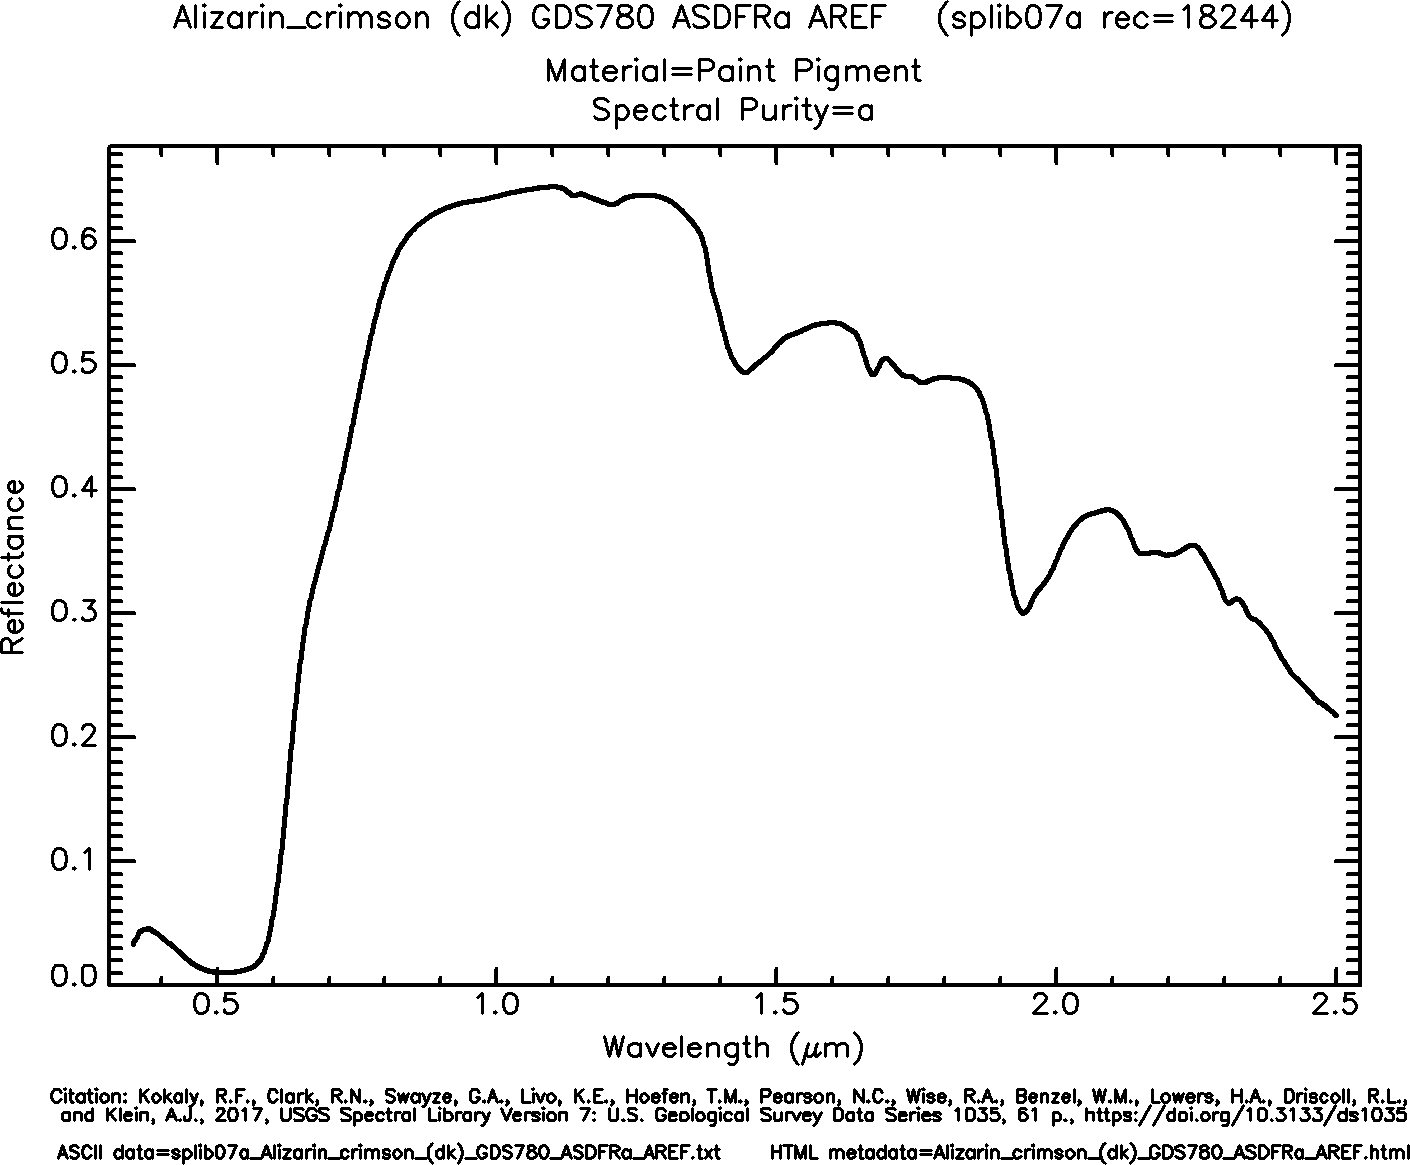
\includegraphics[width=0.8\textwidth]{esempio_firma.png}
    \caption{Firma spettrale dell'alizarina cremisi}
    \label{esempio_firma}
\end{figure}

\subsection{USGS Spectral Library}
Il dataset scelto per verificare la fattibilità della classificazione di oggetti tramite la loro firma spettrale è stato quello dello United States
Geological Survey, un'agenzia scientifica del governo degli Stati Uniti d'America.
Il dataset è denominato USGS Spectral Library Version 7.
Questo insieme di dati è stato raccolto nel corso degli anni dai ricercatori dell'ente menzionato facendo rilevazioni su migliaia di materiali in laboratorio,
usando diversi tipi di spettrometri, i quali coprono lunghezze d'onda che vanno dall'ultravioletto all'infrarosso (da \unit{0.2}{\micro\meter} a \unit{200}{\micro\meter}).
Gli strumenti usati, in dettaglio, sono:
\begin{itemize}
    \item Beckman\textsuperscript{TM} 5270, il quale copre l'intervallo spettrale dai 0.2 ai 3 \micro\meter;
    \item i modelli standard, high-resolution (hi-res) e high-resolution Next Generation (hi-resNG) della Analytical Spectral Devices (ASD);
          che coprono tutti dai 0.35 ai 2.5 \micro\meter;
    \item Nicolet\textsuperscript{TM} Fourier Transform Infra-Red (FTIR) che copre dai 1.12 ai 216 \micro\meter;
    \item NASA Airborne Visible/Infra-Red Imaging Spectrometer (AVIRIS) il quale copre dai 0.37 ai 2.5 \micro\meter.
\end{itemize}
Le classi di materiale prese in considerazione sono:
\begin{itemize}
    \item minerali;
    \item terreno (incluso rocce e minerali);
    \item rivestimenti su superfici rocciose;
    \item liquidi;
    \item composti organici;
    \item materiali artificiali;
    \item vegetazione e altri materiali biologici.
\end{itemize}
Una caratteristica degna di nota del dataset è che in corrispondenza di lunghezze d'onda il cui valore di riflettanza fosse stato eccessivamente sporcato da gas atmosferici questo è stato impostato a $-1.23 \cdot 10^{34}$, il quale corrisponde al "deleted channel" del software SPECPR (SPECtrum Processing Routines). Di conseguenza questi valori dovranno essere rimossi, per evitare che il modello prenda degli input inconsistenti durante il processo di allenamento.\\
In totale sono stati presi in considerazione 61453 esempi, con la distribuzione in classi riportata in figura \ref{distr_esempi}. Come si può notare dal grafico, ci troviamo in presenza di dati sbilanciati, con più della metà appartenente alla classe di rocce e minerali, una minima parte appartenente a rivestimenti e liquidi (in totale $1.5\%$), e i restanti esempi circa equidistribuiti tra le restanti classi.

\begin{figure}
    \centering
    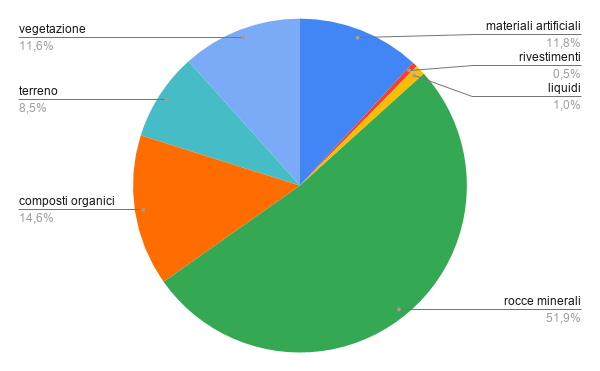
\includegraphics[width=0.8\textwidth]{distribuzione_dataset.png}
    \caption{Distribuzione esempi del dataset in classi}
    \label{distr_esempi}
\end{figure}

\subsection{Elaborazione dei dati}
In primo luogo è stato necessario formattare i dati contenuti nel dataset in modo che fossero poi pronti come input per il modello di machine learning. Originariamente questi erano contenuti in file formato \verb|.txt| codificati in ASCII. In particolare erano suddivisi in cartelle in base allo spettrometro usato nelle rilevazioni e all'anno in cui sono state effettuate. Dentro ognuna di queste poi, vi era una cartella per ogni classe di materiale, contenente le lo spettro luminoso di ogni materiale. Il file con la lunghezza d'onda era comune per tutti i materiali. Per questa attività si sono realizzati degli script in linguaggio Python, i quali rimuovevano caratteri come spazi e stringhe. Il risultato, per ogni cartella, è un file \verb|data.txt| in cui ogni linea identifica una rilevazione. In particolare il primo numero intero $n \in \{ 0 .. 6 \}$ identifica la classe di appartenenza secondo questa mappa:
\begin{itemize}
    \item $0 \rightarrow$ materiali artificiali
    \item $1 \rightarrow$ rivestimenti
    \item $2 \rightarrow$ liquidi
    \item $3 \rightarrow$ rocce minerali
    \item $4 \rightarrow$ composti organici
    \item $5 \rightarrow$ terreno
    \item $6 \rightarrow$ vegetazione
\end{itemize}
Successivamente ci sono $k$ numeri che rappresentano lo spettro luminoso, seguiti da altrettanti per le lunghezze d'onda corrispondenti. Più in dettaglio, il numero n-esimo nell'array dello spettro luminoso corrisponde all'n-esimo nell'array delle lunghezze d'onda. Il valore $k$ dipende dallo strumento usato per la rilevazione.\\
Vista l'eterogeneità delle righe del file, le quali hanno lunghezze diverse a causa della diversità delle misurazioni effettuate, si è resa necessaria una fase di uniformazione. Questa è stata effettuata usando il software proprietario MATLAB\_R2021A, lo script è riportato in \ref{script_matlab}.

\lstset{
    commentstyle=\color{ForestGreen},
    language=Matlab,
    caption=Script Matlab per l'elaborazione del dataset,
    label=script_matlab
}
\begin{lstlisting}
    clear;
    clc;
    dataset = fopen('dataset.txt', 'r');
    y_file = fopen('y.txt', 'w');
    x_file = fopen('x.txt', 'w');
    current = fgetl(dataset);
    while ischar(current)
        % converting txt line to array
        splitted = split(current, ';');
        wavelengths = str2double(split(splitted(3), ','));
        reflectance = str2double(split(splitted(2), ','));
        
        % removing dirty channels
        idx = ismember(reflectance, 1.23e34);
        reflectance(idx) = [];
        wavelengths(idx) = [];
        
        % interpolation
        x = linspace(wavelengths(1), wavelengths(end), 2000);
        s = spline(wavelengths, reflectance, x);
        
        % writing result to files
        fprintf(y_file, '%d\n', splitted(1));
        fprintf(x_file, '%f ',s);
        fprintf(x_file, '\n');
        
        % getting next line
        current = fgetl(dataset);
    end
    fclose(dataset);
    fclose(y_file);
    fclose(x_file);
\end{lstlisting}
dove il file \verb|dataset.txt| è l'unione dei file generati per ogni cartella in precedenza con lo script Python.
Ogni linea viene divisa nelle tre parti prima descritte, inoltre dai valori di riflettanza e lunghezza d'onda vengono rimossi i canali con valori eliminati a causa di errori troppo elevati nella rilevazione.
Successivamente i valori vengono interpolati con una spline cubica e portati ad un'unica dimensionalità di 2000 punti. Quello che interessa per identificare un oggetto tramite la firma spettrale, cosi come dedotto dall'incontro con l'esperto in geologia, è l'andamento del valore di riflettanza, ad esempio particolari picchi o oscillazioni. Di conseguenza non è fondamentale che i valori di lunghezza d'onda siano esattamente gli stessi, perciò l'interpolazione avviene considerando gli estremi dell'intervallo delle lunghezze d'onda per ogni esempio. È stato scelto questo particolare metodo di interpolazione visto che assicura la convergenza anche con nodi equispaziati ed è stabile, al contrario di quello polinomiale.\\
L'output di questo script sono i due file \verb|x.txt| e \verb|y.txt|, i quali sono pronti ad essere caricati in linguaggio Python per usarli come input del modello di apprendimento automatico.

\section{Sviluppo del modello di machine learning}
Tra le varie possibilità che i framework per i machine learning offrono al giorno d'oggi si sono fatte alcune considerazioni sui seguenti, facendo ricadere la scelta finale sulle reti neurali MLP (Multi-Layer-Perceptron).

\subsection{Strumento adottato}
Per questa parte del progetto ci si è affidati allo strumento offerto as-a-service Google Colaboratory, il quale è un'implementazione del progetto Jupyter con base di archiviazione Google Drive.
I Jupyter notebook sono un'insieme di script python intervallati da testo descrittivo.
Il vantaggio nell'utilizzo di questo strumento è innanzitutto la possibilità di usare hardware come GPU offerte gratuitamente dall'infrastruttura cloud di Google per eseguire gli script. Inoltre è possibile eseguire una parte di codice alla volta o tutto insieme, mantenendo le variabili in memoria RAM per tutta la durata della sessione. È possibile quindi allenare la rete e successivamente eseguire dei test sul modello allenato, stampare grafici con le curve di apprendimento o salvare il modello allenato su Google Drive.

\subsection{Scelta del modello}
\subsubsection{k-nearest-neighbour}
Una prima considerazione è stata fatta in base al successivo utilizzo del modello allenato: questo dovrà essere interpellato per effettuare predizioni in real time, dunque il tempo di risposta dovrà essere costante. Ne segue che modelli basati su \textbf{k-nearest-neighbour} non possono essere adottati, in quanto il tempo di esecuzione dell'algoritmo di predizione ricade nella classe di complessità $\theta (n)$ dove $n$ è il numero di esempi classificati. Questo perché la classificazione dei nuovi esempi si basa sul calcolo della distanza dagli esempi nel training set in uno spazio d-dimensionale (dove $d$ è il numero di features, nel nostro caso 2000), successivamente si trovano i $k$ esempi più vicini a quello da classificare, tra questi si guarda la classe più frequente. Una volta che un esempio è classificato viene usato nelle predizioni successive, dunque il tempo per il calcolo delle distanze aumenta. Questo è impraticabile in un sistema real-time, il quale richiede che i tempi di risposta siano costanti, ne segue la decisione prima menzionata.

\subsubsection{Support Vector Machines}
Questo tipo di modello è stato preso in considerazione visto che è un algoritmo di apprendimento supervisionato usato spesso per compiti di classificazione. È un modello di classificazione lineare ma può essere usato efficientemente per effettuare classificazioni non lineari usando il \textit{kernel trick}. Inoltre è molto efficace in spazi a molte dimensioni.
Per l'implementazione ci si è affidati alla libreria scikit-learn, la quale offre dei modelli per la classificazione con le seguenti classi:
\begin{itemize}
    \item SVC: Support Vector Classification, la cui implementazione è basata sulla libreria \verb|libsvm| scritta in linguaggio C++, dunque offre la velocità di un linguaggio compilato. Il tempo di training è nella classe di complessità $\theta (n^2)$ con $n$ il numero di esempi nel set di training, dunque diventa inutilizzabile con le dimensioni del nostro dataset. Questo perché effettua un tipo di classificazione one-vs-one, dunque allena $k \cdot (k-1)/2$ classificatori binari con $k$ il numero di classi;
    \item NuSVC: simile al precedente ma aggiunge un parametro per controllare il numero dei support vectors;
    \item LinearSVC: questo è stato il tipo di modello che si è provato ad utilizzare nel nostro caso. A differenza dei precedenti allena dei classificatori di tipo one-vs-all, ovvero un classificatore per ogni classe. Ne segue che non c'è più la complessità quadratica per l'algoritmo di allenamento. È simile alla classe SVC con parametro nel costruttore \verb|kernel='linear'|, tuttavia la sua implementazione si basa sulla libreria \verb|liblinear|, anch'essa scritta in C++ ma che scala meglio all'aumentare delle dimensioni del dataset.
\end{itemize}
Il modello è stato inserito in una pipeline che prevedesse uno step precedente per la normalizzazione delle features tramite la classe \verb|StandardScaler| offerta dalla stessa libreria. Si è applicata inoltre la procedura di hold-out, che prevede la suddivisione del dataset in due parti, training e validation set. La dimensione scelta per il primo è $80\%$, per il secondo il restante $20\%$, la suddivisione è stata effettuata in modo casuale usando la funzione \verb|train_test_split| offerta dalla stessa libreria.\\
Successivamente il modello allenato è stato testato valutando l'accuratezza nell'effettuare le predizioni sul set di validazione, le prove hanno dato esito negativo visto che non si è superato il $62\%$ in questa metrica.

\subsubsection{Multi Layer Perceptron}
In seguito all'insuccesso riportato con le Support Vector Machines con kernel lineare si è deciso di passare ad algoritmi di deep learning. Si sono prese in considerazione le classiche rete neurali artificiali a strati, adottando la libreria Pytorch per l'implementazione, visto che permette di addestrare la rete su GPU rendendo questo processo significativamente più veloce.
L'unità fondamentale in questo tipo di modello è il percettrone (neurone), il quale rappresenta un modello di machine learning semplice, dotato di una funzione e di un valore di attivazione. Ogni unità è connessa a tutte quelle nello strato successivo e ad ogni connessione è associato un peso (appreso tramite backpropagation). Ad ogni strato è inoltre associato un bias. Per calcolare il valore di attivazione di ogni neurone si effettua un'operazione lineare che vede la somma tra il valore di attivazione del neurone nel layer precedente moltiplicato per il peso della connessione, a cui si somma infine il bias del layer (anch'esso appreso automaticamente). Questo è definito passo di forward, l'idea di funzionamento viene meglio presentata nell'algoritmo \ref{grad_desc_backprop}. Le notazioni adottate sono le seguenti:
\begin{itemize}
    \item $\theta^{(l)}$ indica il vettore dei pesi delle connessioni tra il layer $l$ e $l+1$. Questo è preso dalla matrice dei pesi $\theta$;
    \item $a^{(l)}$ indica i valori di attivazione dei neuroni al layer $l$, risultati dell'operazione $f(z^{(l)})$ dove $f$ è la funzione di attivazione scelta e $z^{(l)}$ il risultato dell'operazione lineare effettuata tra i valori di attivazione dei neuroni al layer precedente, i pesi nella matrice $\theta$ e i valori di bias;
    \item $\delta^{(l)}$ è la variazione desiderata per i valori di attivazione ottenuti al layer $l$.
\end{itemize}
Il layer di output sarà composto da 7 percettroni, ognuno dei quali indica la probabilità che un certo esempio appartenga o meno alla classe rappresentata (infatti nel dataset ci sono 7 classi di oggetti).

\begin{algorithm}
    \caption{Gradient descent with backpropagation}
    \label{grad_desc_backprop}
    \begin{algorithmic}
        \State Training samples $\{ (x^{(1)}, y^{(1)}), \dotso, (x^{(m)}, y^{(m)}) \}$
        \State Initialize $\theta^{l}$ with random values close to zero, e.g. $\in [-\epsilon, +\epsilon]$
        \For{all epochs}
            \State Initialize $\Delta_{ij}^{(l)} = 0$ $\forall i, j, l$ \Comment Accumulatori per calcolo derivata
            \For{k=1 to m}
                \State set $a^{(1)} = x^{(k)}$ \Comment imposto primo layer da input
                \For{l=2 to L}
                    \State compute $a^{(l)}$ \Comment forward propagation
                \EndFor
                \State compute $\delta^{(L)} = a^{(L)} - y^{(k)}$
                \For{l=L-1 down to 2}
                    \State compute $\delta^{(l)} = ((\theta^{(l)})^T \cdot \delta^{l+1}) \ .* f'(z^{(l)})$ \Comment backpropagation
                \EndFor
                \State compute gradients $\Delta^{(l)} = \Delta^{(l)} + \delta^{(l+1)} \cdot (a^{(l)})^T$
            \EndFor
            \State compute $D^{(l)}_{ij} = 
            \begin{cases}
                \frac{1}{m} \cdot (\Delta^{(l)}_{ij} + \lambda \theta^{(l)}_{ij}) $ if $ j \neq 0 \\
                \frac{1}{m} \cdot \Delta^{(l)}_{ij} $ if $ j = 0
            \end{cases}$
            \State $\theta^{(l)}_{ij} = \theta^{(l)}_{ij} - \eta \cdot D_{ij}^{(l)}$
        \EndFor
    \end{algorithmic}
\end{algorithm}

\subsection{Implementazione e validazione}
Come prima accennato, si è fatto largo uso di Pytorch nell'implementazione della rete. In particolare si è definita la classe \verb|MLP| che eredita da \verb|nn.Module|, ovvero la classe base per ogni modello di rete neurale. Non sono stati ridefiniti metodi degni di nota, se non la possibilità di invocare il costruttore modificando gli iperparametri della rete in modo semplice. Inoltre si è adottata la variante Adam di gradient descent, che assicura una convergenza più veloce. Gli iperparametri adottati sono i seguenti:
\begin{itemize}
    \item \verb|layers size:| $[2000, 1500, 500, 7]$, indica il numero di neuroni per ogni layer. In questo caso abbiamo una rete a 3 strati (2 nascosti e uno di output), il primo strato di input è composto da 2000 percettroni, uno per ogni dimensione degli esempi. 1500 percettroni per il primo hidden layer e 500 per il secondo. Infine 7 unità per il layer di output, per il motivo prima riportato;
    \item \verb|activation:| come funzione di attivazione dei neuroni si è scelta la funzione rectifier (ReLU) definita come $f(x) = x^+ = max(0,x)$ (vedi figura \ref{relu_func});
    \begin{figure}
        \centering
        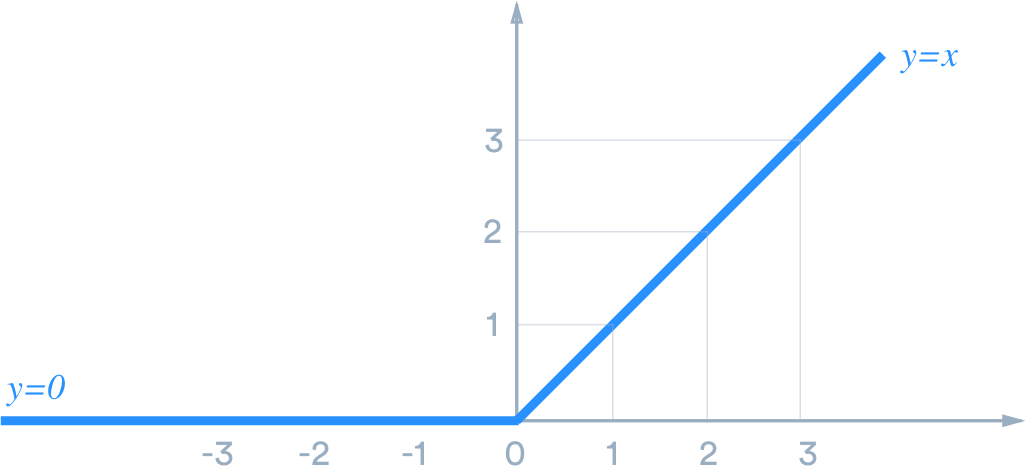
\includegraphics[width=0.6\textwidth]{relu.png}
        \caption{Funzione ReLU}
        \label{relu_func}
    \end{figure}
    \item \verb|learning rate:| $10^{-4}$, questo è il parametro $\eta$ usato in gradient descent. Se troppo basso l'algoritmo diventa lento, se troppo alto si rischia di fare overshooting (saltare il minimo della funzione di costo) o addirittura divergere;
    \item \verb|epochs:| 50, indica il numero di epoche nell'algoritmo di apprendimento;
    \item \verb|init kind:| xavier, indica come inizializzare i pesi $\theta$ delle connessioni tra i neuroni;
    \item \verb|dropout rate:| 0.2 indica che il $20\%$ dei neuroni viene disattivato scegliendo casualmente. È un tipo di regolarizzazione e serve a ridurre overfitting.
\end{itemize}
Le prestazioni ottenute con i parametri sopra elencate sono riportate nelle figure \ref{cross_entropy_loss_plot} e \ref{accuracy_plot}. 

\begin{figure}
    \centering
    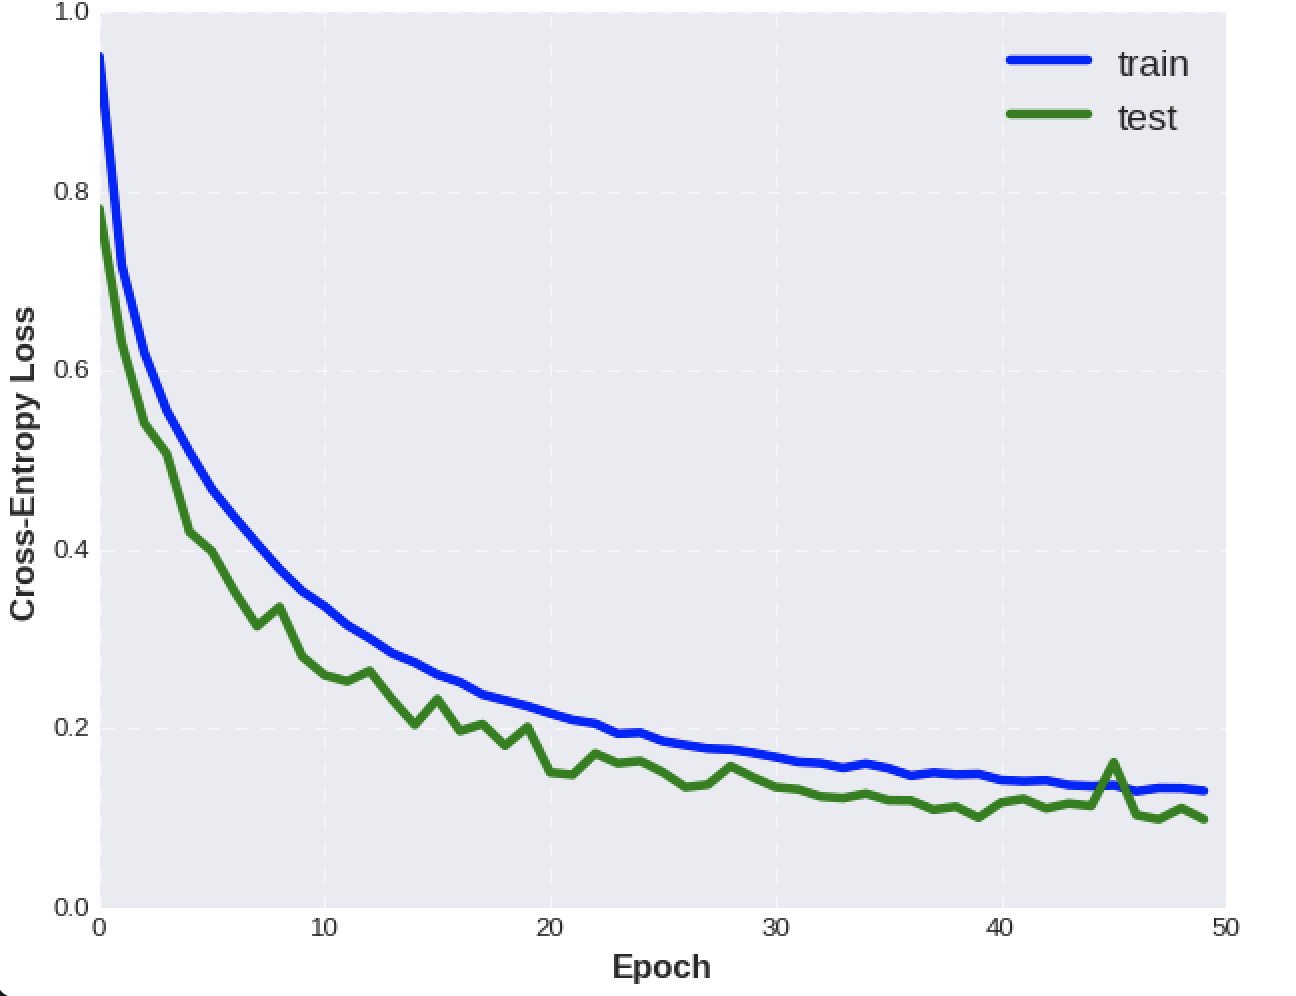
\includegraphics[width=0.9\textwidth]{cross_entropy_loss.png}
    \caption{Cross Entropy Loss plot}
    \label{cross_entropy_loss_plot}
\end{figure}

\begin{figure}
    \centering
    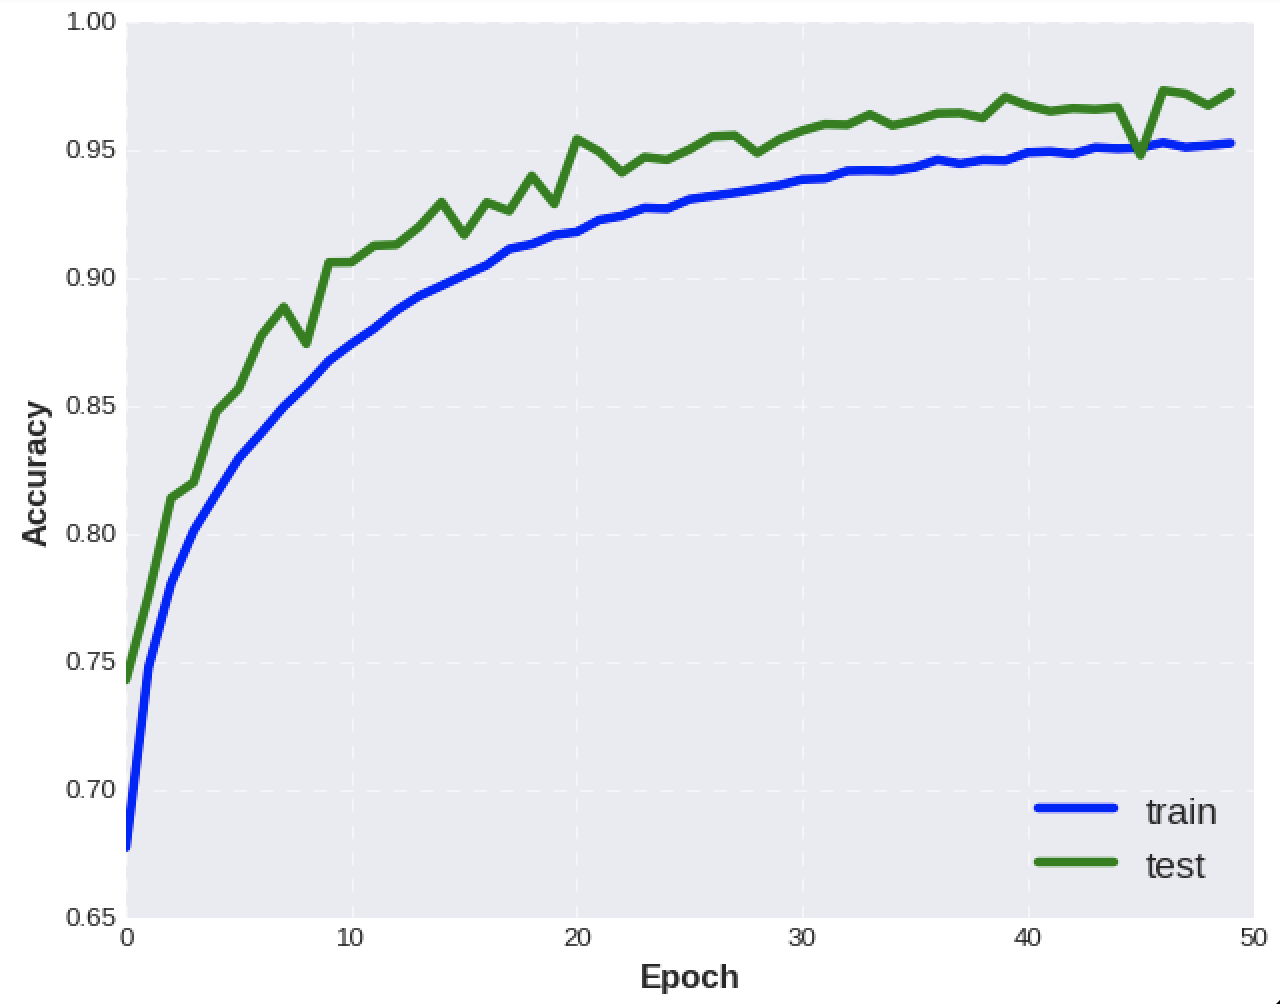
\includegraphics[width=0.9\textwidth]{accuracy.png}
    \caption{Accuracy plot}
    \label{accuracy_plot}
\end{figure}
Nella prima si vede come la funzione di costo diminuisca con l'avanzare delle epoche di apprendimento, nella seconda si può notare l'aumentare dell'accuratezza anche nel set di test.\\
Il dataset è stato suddiviso in tre insiemi disgiunti:
\begin{itemize}
    \item training set: usato per la fase di apprendimento è composto dal $70\%$ degli esempi;
    \item test set: usato nella fase di apprendimento per verificate l'andamento alla fine di ogni epoca, è composto dal $15\%$ degli esempi;
    \item validation set: usato alla fine della fase di apprendimento per valutare le prestazioni del modello allenato, è composto dal restante $15\%$ degli esempi.
\end{itemize}
Come si può notare dal grafico \ref{accuracy_plot}, il valore di accuratezza raggiunto alla cinquantesima epoca è intorno al $97\%$. I risultati di predizione sul set di validazione mostrano un'accuratezza del $98.23\%$, per un totale di 9055 esempi su 9218 classificati correttamente.

\section{Esposizione API per predizioni}
Una volta allenata la rete neurale, questa è stata serializzata in un file attraverso la libreria \verb|pickle| presente nativamente nel linguaggio Python. Per interfacciarla con il codice che calcola la traiettoria del drone e si interfaccia con esso, è stato necessario scegliere tra una delle seguenti opzioni:
\begin{itemize}
    \item utilizzare i servizi di tipo serverless offerti da un'infrastruttura cloud, ad esempio quelli di Amazon Web Services Lambda e S3;
    \item utilizzare un servizio ottimizzato per il machine learning di nome Amazon SageMaker;
    \item sviluppare un web server da ospitare su una macchina locale oppure remota presa in affitto da tipici servizi di hosting web, ad esempio Aruba.
\end{itemize}
La prima opzione è stata prontamente scartata, visto che un'architettura serverless è incompatibile con il nostro caso d'uso. In particolare il modello serializzato ha un peso approssimativo di 90 MB, dunque ad ogni chiamata dell'API è richiesto il caricamento di questo. Una ripresa a freddo ad ogni predizione aumenterebbe notevolmente i costi fatturati dal servizio.\\
La seconda opzione è stata presa in considerazione inizialmente, tuttavia visto il tempo ristretto per le attività di stage e le difficoltà incontrate nel cercare di caricare il modello, si è deciso di accantonare anche questa possibilità.\\
La scelta è ricaduta quindi sulla classica architettura client-server, permettendo di caricare il modello allenato solo una volta all'avvio del server, avendo quindi tempi di risposta molto brevi grazie alla ripresa a caldo. Inoltre i costi di un servizio del genere sono ridotti e non è richiesta la scalabilità dell'applicazione.\\
Per la realizzazione di questo si è usato il web framework \verb|Flask|, ovvero un modulo Python che permette di sviluppare applicazioni web in modo molto semplice. Il server, se avviato in locale, si mette in ascolto sulla porta 5000 e risponde a chiamate POST del protocollo HTTP. Per ottenere una risposta valida è necessario che nel corpo della richiesta venga inclusa una firma spettrale composta da 2000 elementi.\\
All'avvio il server effettua la deserializzazione del modello utilizzando l'apposita classe \verb|CPU_Unpickler|, la quale si basa ovviamente sulla libreria usata per la serializzazione. Questa è fondamentale visto che la rete è stata addestrata su schede grafiche, dunque si aspetta di effettuare predizioni con lo stesso hardware. La classe infatti rende il modello utilizzabile su macchine con solo CPU, ovvero tutte quelle offerte dai comuni servizi di hosting, trasformandolo in fase di deserializzazione.             % dataset e ML
% !TEX encoding = UTF-8
% !TEX TS-program = pdflatex
% !TEX root = ../tesi.tex

%**************************************************************
\chapter{Algoritmo per il calcolo della traiettoria}
\label{cap:business-logic}
%**************************************************************

\intro{In questa sezione si documenterà la realizzazione della business logic per il calcolo della traiettoria e l'interfacciamento con il drone.}\\

%**************************************************************

\section{Strumenti utilizzati}
Il linguaggio scelto per sviluppare questa componente della Proof of Concept è Java nella versione 11. Si è usato l'IDE IntelliJ IDEA Education, il quale offre un ambiente di sviluppo integrato sia per Java che per Python. In questo modo è stato possibile eseguire il server per le predizioni insieme al modulo del programma in Java che si interfaccia con questo in modo molto semplificato.

\section{Architettura generale}
L'architettura data all'applicazione è quella del monolite a strati, di cui si può vedere una rappresentazione ad alto livello nella figura \ref{fig:layered_architecture}. Il principale vantaggio che si ottiene dall'adozione di questa architettura è alta testabilità: infatti è molto semplice creare delle componenti di mock o addirittura layer interi che sostituiscono quelli reali, al fine di testare gli strati superiori.
    
\begin{figure}
    \centering
    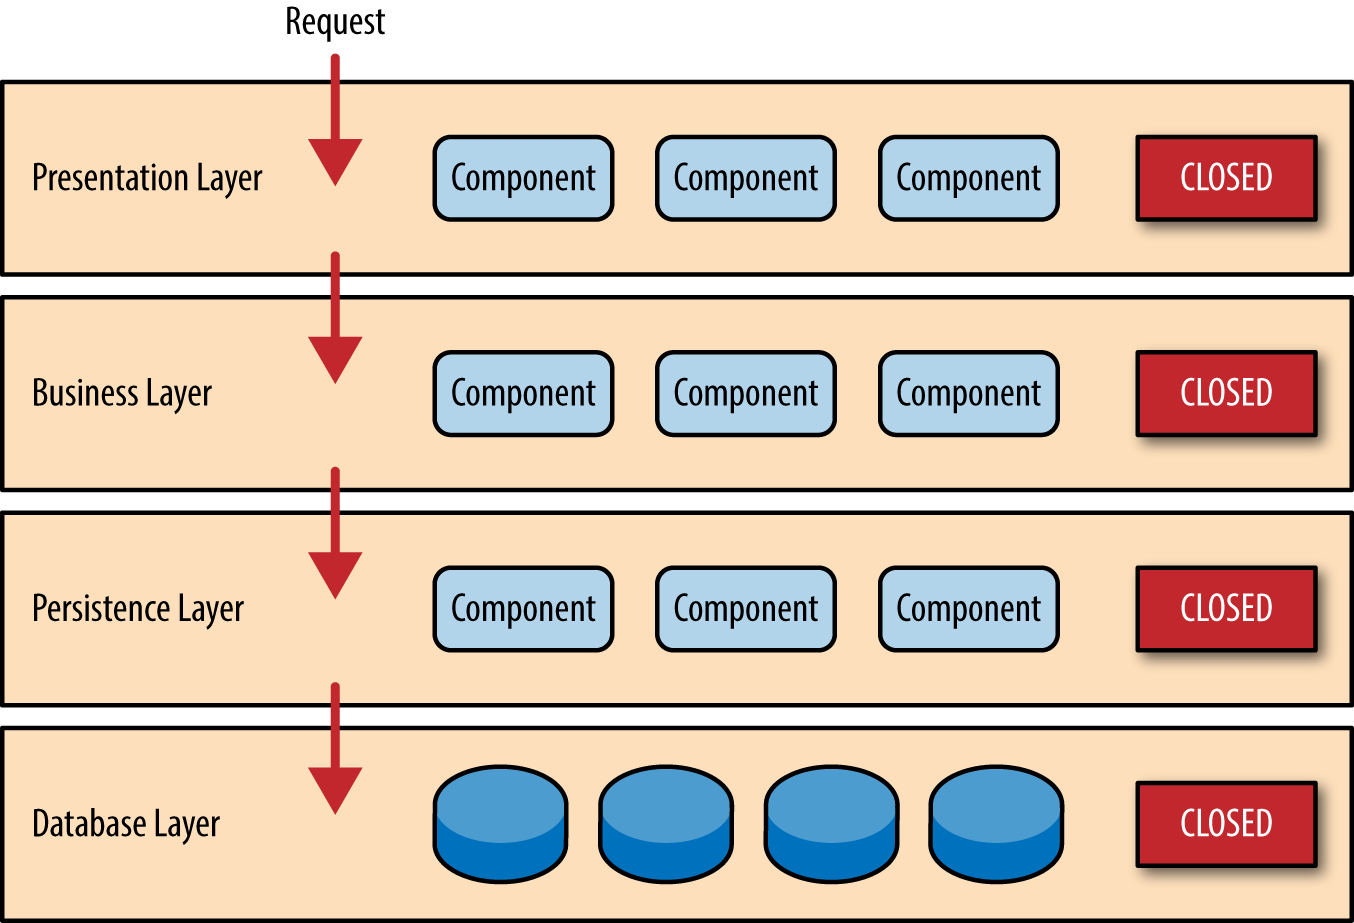
\includegraphics[width=\textwidth]{immagini/layered_archiecture.png}
    \caption{Architettura monolitica a strati}
    \label{fig:layered_architecture}
\end{figure}

\subsection{Strato di persistenza}
Nel nostro caso al posto del Database, alla base, c'è il server che espone la rete neurale per le predizioni. Di conseguenza lo strato di persistenza è l'insieme di quelle classi addette a comporre la richiesta HTTP da inviare all'end-point, le quali sono collocate nel package prediction. In particolare all'interno di questo troviamo la classe NeuralNetworkClient che contiene tra i suoi campi dati un oggetto con il tipo HttpClient, offerta dalla libreria \verb|java.net|. Grazie a questo è possibile esporre nell'interfaccia pubblica della classe il metodo \verb|predict|, il quale prende come parametro una lista contenente i valori dello spettro luminoso (già interpolati in modo che siano uniformi con i valori con cui la rete è stata allenata) e ritorna un valore interno $k \in \{0 .. 6 \}$ che indica la classe di appartenenza tra quelle elencate nel capitolo \ref{cap:machine-learning}. Questo metodo ha inoltre il compito di gestire eventuali eccezioni lanciate durante la chiamata al server, ritornando un valore negativo.\\
È possibile vedere il diagramma delle classi per questo layer nella figura \ref{fig:class_diagram_persistence}.

\begin{figure}
    \centering
    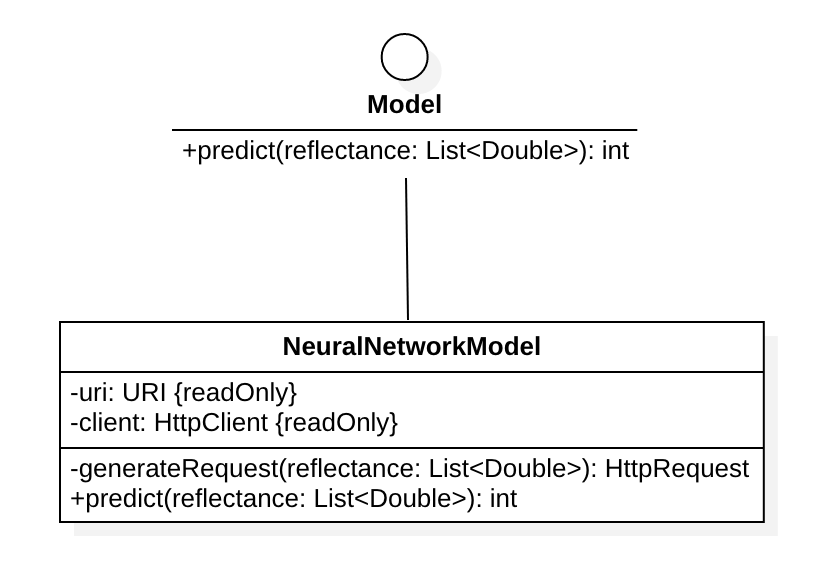
\includegraphics[width=0.8\textwidth]{immagini/model_classes.png}
    \caption{Diagramma delle classi per lo strato di persistenza}
    \label{fig:class_diagram_persistence}
\end{figure}

\subsection{Strato di business}
Salendo, a questo livello, troviamo l'insieme delle classi atte al calcolo del percorso che il drone dovrà eseguire. Si riporta nell'algoritmo \ref{alg:calculate_track} lo pseudocodice per il calcolo del percorso. L'input sono due array paralleli $x$ e $y$ di grandezza $n$ (con $n$ il numero di punti da attraversare) contenenti le coordinate. Possiamo notare come questo problema è riconducibile ad un grafo completo $K_n$, in cui ogni nodo è connesso da un arco a tutti gli altri. Ognuno di questi archi ha un costo di percorrenza che dipende direttamente dalla distanza tra i due punti, espressi in coordinate. Ci troviamo di fronte al problema del commesso viaggiatore.\\
È possibile vedere il diagramma delle classi per questo layer nella figura \ref{fig:class_diagram_business}.

\begin{figure}
    \centering
    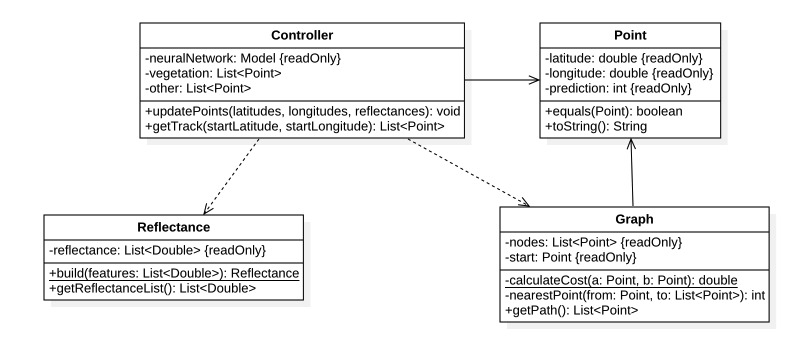
\includegraphics[width=\textwidth]{immagini/business_classes.png}
    \caption{Diagramma delle classi per lo strato di business}
    \label{fig:class_diagram_business}
\end{figure}

\subsubsection{Problema del commesso viaggiatore}
Il nome nasce da una tipica rappresentazione del problema: dato un insieme di città da visitare una ed una sola volta e note le distanze tra queste, trovare il tragitto di minima percorrenza che un commesso viaggiatore deve eseguire per effettuare tutte le consegne e ritornare al punto di partenza. È stato dimostrato che questo problema è \textit{NP-hard}, in quanto non esiste un algoritmo che lo risolva in tempo polinomiale. L'unico metodo di risoluzione efficace è l'enumerazione totale dei possibili percorsi, che ricade nella classe di complessità computazionale $\theta(n!)$.

\subsubsection{Algoritmo euristico di risoluzione}
Per affrontare il problema si è deciso di realizzare un algoritmo euristico, ovvero la cui soluzione prodotta è probabilmente buona ma non ottima.
Come si può notare, il costo computazionale della procedura \verb|nearest_point| è lineare, dunque il costo totale della procedura rientra nella classe di algoritmi $\theta(n^2)$ con consumo di memoria costante. Considerando che nell'applicazione reale il valore di $n$ non raggiungerà mai valori elevati, il risultato è accettabile. Inoltre è possibile ottimizzare questo algoritmo durante l'implementazione rimuovendo i punti già inclusi nel cammino dagli array $x$ e $y$ invece di porre le coordinate a infinito.
Per il calcolo della distanza tra due coordinate, si è deciso di non considerare la curvatura terrestre, visto che nell'applicazione reale i punti saranno molto vicini tra loro e che il software realizzato è solo una Proof of Concept.

\begin{algorithm}
    \caption{Algoritmo per il calcolo del percorso}
    \label{alg:calculate_track}
    \begin{algorithmic}
        \Require array $x[1 \dotso n]$ e $y[1 \dotso n]$ senza valori duplicati
        \Require $x\_start \notin x$ e $y\_start \notin y$
        \Ensure $x\_path[1 \dotso n+1]$ e $y\_path[1 \dotso n+1]$
        \State Inizializza array $x\_path[1 \dotso n+1]$, $y\_path[1 \dotso n+1]$
        \State $x\_prev \leftarrow x\_start$
        \State $y\_prev \leftarrow y\_start$
        \For{$i \leftarrow 1$ to $n$}
            \State $next \leftarrow \verb|nearest_point|(x\_prev,\  y\_prev,\  x,\  y)$
            \Comment Algoritmo \ref{alg:nearest_point}
            \State $x\_path[i] \leftarrow x[next]$
            \State $y\_path[i] \leftarrow y[next]$
            \State $x[next] \leftarrow \infty$
            \State $y[next] \leftarrow \infty$
            \State $x\_prev \leftarrow x[i]$
            \State $y\_prev \leftarrow y[i]$
        \EndFor
        \State $x\_path[n+1] \leftarrow x\_start$ \Comment Punto di arrivo
        \State $y\_path[n+1] \leftarrow y\_start$
        \State \Return $(x\_path , y\_path)$
    \end{algorithmic}
\end{algorithm}

\begin{algorithm}
    \caption{Procedura nearest point}
    \label{alg:nearest_point}
    \begin{algorithmic}
        \Require $x\_from$, $y\_from$ il punto di partenza
        \Require $x\_to[1 \dotso n]$, $y\_to[1 \dotso n]$ array con le $n$ destinazioni possibili differenti
        \Ensure $minIndex$ l'indice della posizione più vicina
        \State $minIndex \leftarrow -1$
        \State $minDistance \leftarrow \infty$
        \For{$i \leftarrow 1$ to $n$}
            \State $distance \leftarrow \sqrt{(x\_from - x\_to[i])^2 + (y\_from - y\_to[i])^2}$
            \If{$distance < minDistance$}
                \State $minDistance \leftarrow distance$
                \State $minIndex \leftarrow i$
            \EndIf
        \EndFor
        \State \Return $minIndex$
    \end{algorithmic}
\end{algorithm}

\subsection{Strato di presentazione}
Questo livello ha il compito di esporre tutto il monolite all'esterno.
Va premesso che il drone che andrà ad interfacciarsi con questo software avrà una scheda Arduino, dunque in grado di effettuare chiamate HTTP ad un end-point indicato grazie al linguaggio C++.
Nel nostro specifico caso si tratta di esporne tre:
\begin{itemize}
    \item \verb|/track|: questo risponde a chiamate HTTP di tipo GET, viene invocato dal drone quando ha bisogno di conoscere il tracciato che deve percorrere;
    \item \verb|/data|: questo risponde a chiamate HTTP di tipo POST, viene invocato dal drone quando ha fatto delle rilevazioni con lo spettrometro e le invia al software in modo che il percorso di aggiorni. La risposta può essere un successo o un fallimento;
    \item \verb|/perimeter|: risponde a chiamate HTTP di tipo PATCH, serve a impostare il perimetro di sorvolo del drone.
\end{itemize}
È possibile vedere il diagramma delle classi per questo layer nella figura \ref{fig:class_diagram_presentation}. Le API sono state documentate seguendo lo standard OpenAPI 3.0.0.

\begin{figure}
    \centering
    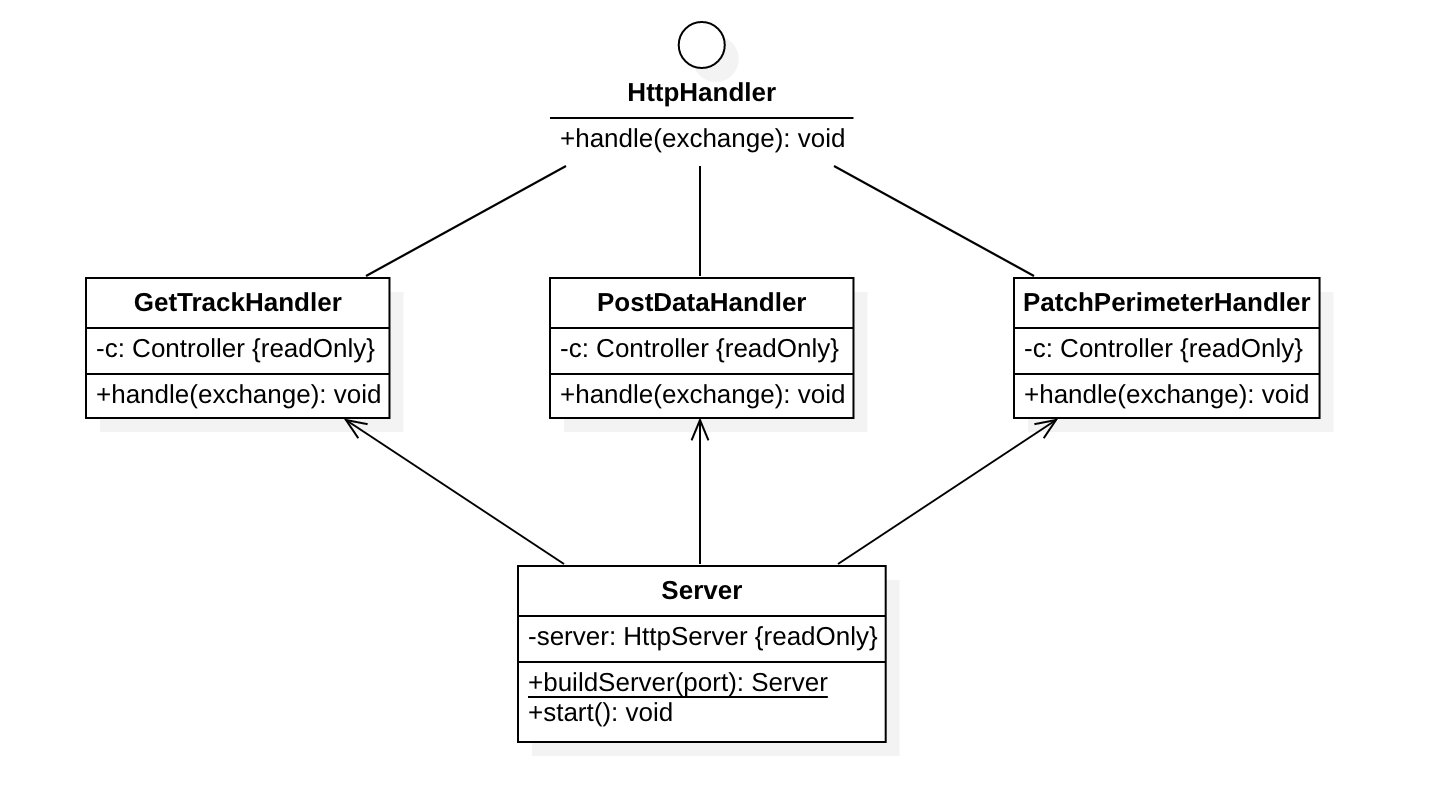
\includegraphics[width=0.8\textwidth]{immagini/presentation_classes.png}
    \caption{Diagramma delle classi per lo strato di presentazione}
    \label{fig:class_diagram_presentation}
\end{figure}             % business logic
% !TEX encoding = UTF-8
% !TEX TS-program = pdflatex
% !TEX root = ../tesi.tex

%**************************************************************
\chapter{Valutazione retrospettiva e conclusioni}
\label{cap:conclusione}
%**************************************************************

\intro{Breve introduzione al capitolo}             % conclusioni
\appendix                               
% !TEX encoding = UTF-8
% !TEX TS-program = pdflatex
% !TEX root = ../tesi.tex

%**************************************************************
\chapter{Appendice A}
%**************************************************************

\epigraph{Citazione}{Autore della citazione}



             % Appendice A

%**************************************************************
% Materiale finale
%**************************************************************
\backmatter
\printglossaries
% !TEX encoding = UTF-8
% !TEX TS-program = pdflatex
% !TEX root = ../tesi.tex

%**************************************************************
% Bibliografia
%**************************************************************

\cleardoublepage
\chapter{Bibliografia}

\nocite{*}
% Stampa i riferimenti bibliografici
\printbibliography[heading=subbibliography,title={Riferimenti bibliografici},type=book]

% Stampa i siti web consultati
\printbibliography[heading=subbibliography,title={Siti web consultati},type=online]


\end{document}
